\documentclass[10pt]{article}
\usepackage[utf8]{inputenc}
\usepackage[T1]{fontenc}
\usepackage{amsmath}
\usepackage{amsfonts}
\usepackage{amssymb}
\usepackage[version=4]{mhchem}
\usepackage{stmaryrd}
\usepackage{graphicx}
\usepackage[export]{adjustbox}
\graphicspath{ {./images/} }
\usepackage{bbold}

\begin{document}
\section*{MATHEMATICS}
\section*{SECTION-A}
\begin{enumerate}
  \setcounter{enumi}{60}
  \item If \(\phi(\mathrm{x})=\frac{1}{\sqrt{\mathrm{x}}} \int_{\frac{\pi}{4}}^{\mathrm{x}}\left(4 \sqrt{2} \sin \mathrm{t}-3 \phi^{\prime}(\mathrm{t})\right) \mathrm{dt}, \mathrm{x}>0\), then \(\phi^{\prime}\left(\frac{\pi}{4}\right)\) is equal to :\\
(1) \(\frac{8}{\sqrt{\pi}}\)\\
(2) \(\frac{4}{6+\sqrt{\pi}}\)\\
(3) \(\frac{8}{6+\sqrt{\pi}}\)\\
(4) \(\frac{4}{6-\sqrt{\pi}}\)
\end{enumerate}

Official Ans. by NTA (3)\\
Allen Ans. (3)\\
Sol. \(\phi^{\prime}(\mathrm{x})=\frac{1}{\sqrt{\mathrm{x}}}\left[\left(4 \sqrt{2} \sin \mathrm{x}-3 \phi^{\prime}(\mathrm{x})\right) .1-0\right]-\frac{1}{2} \mathrm{x}^{-3 / 2}\)\\
\(\int_{\frac{\pi}{4}}^{\mathrm{x}}\left(4 \sqrt{2} \sin \mathrm{t}-3 \phi^{\prime}(\mathrm{t})\right) \mathrm{dt}\),\\
\(\phi^{\prime}\left(\frac{\pi}{4}\right)=\frac{2}{\sqrt{\pi}}\left[4-3 \phi^{\prime}\left(\frac{\pi}{4}\right)\right]+0\)\\
\(\left(1+\frac{6}{\sqrt{\pi}}\right) \phi^{\prime}\left(\frac{\pi}{4}\right)=\frac{8}{\sqrt{\pi}}\)\\
\(\phi^{\prime}\left(\frac{\pi}{4}\right)=\frac{8}{\sqrt{\pi}+6}\)

\section*{TEST PAPER WITH SOLUTION}
\begin{enumerate}
  \setcounter{enumi}{61}
  \item If a point \(\mathrm{P}(\alpha, \beta, \gamma)\) satisfying \((\alpha \beta \gamma)\left(\begin{array}{ccc}2 & 10 & 8 \\ 9 & 3 & 8 \\ 8 & 4 & 8\end{array}\right)=\left(\begin{array}{lll}0 & 0 & 0\end{array}\right)\) lies on the plane \(2 \mathrm{x}+4 \mathrm{y}+3 \mathrm{z}=5\), then \(6 \alpha+9 \beta+7 \gamma\) is equal to:\\
(1) -1\\
(2) \(\frac{11}{5}\)\\
(3) \(\frac{5}{4}\)\\
(4) 11
\end{enumerate}

Official Ans. by NTA (4)\\
Allen Ans. (4)\\
Sol. \(2 \alpha+4 \beta+3 \gamma=5\)\\
\(2 \alpha+9 \beta+8 \gamma=0\)\\
\(10 \alpha+3 \beta+4 \gamma=0\)\\
\(8 \alpha+8 \beta+8 \gamma=0\)

Subtract (4) from (2)\\
\(-6 \alpha+\beta=0\)\\
\(\beta=6 \alpha\)

From equation (4)\\
\(8 \alpha+48 \alpha+8 \gamma=0\)\\
\(\gamma=-7 \alpha\)

From equation (1)\\
\(2 \alpha+24 \alpha-21 \alpha=5\)\\
\(5 \alpha=5\)\\
\(\alpha=1\)\\
\(\beta=+6, \quad \gamma=-7\)\\
\(\therefore 6 \alpha+9 \beta+7 \gamma\)\\
\(=6+54-49\)\\
\(=11\)\\
63. Let \(\mathrm{a}_{1}, \mathrm{a}_{2}, \mathrm{a}_{3}, \ldots\). be an A.P. If \(\mathrm{a}_{7}=3\), the product \(\mathrm{a}_{1} \mathrm{a}_{4}\) is minimum and the sum of its first n terms is zero, then \(\mathrm{n}!-4 \mathrm{a}_{\mathrm{n}(\mathrm{n}+2)}\) is equal to:\\
(1) 24\\
(2) \(\frac{33}{4}\)\\
(3) \(\frac{381}{4}\)\\
(4) 9

\section*{Official Ans. by NTA (1)}
\section*{Allen Ans. (1)}
Sol. \(\mathrm{a}+6 \mathrm{~d}=3\),\\
\(\mathrm{Z}=\mathrm{a}(\mathrm{a}+3 \mathrm{~d})\)\\
\(=(3-6 \mathrm{~d})(3-3 \mathrm{~d})\)\\
\(=18 \mathrm{~d}^{2}-27 \mathrm{~d}+9\)\\
Differentiating with respect to d\\
\(\Rightarrow 36 \mathrm{~d}-27=0\)\\
\(\Rightarrow \mathrm{d}=\frac{3}{4}\), from (1) \(\mathrm{a}=\frac{-3}{2},(\mathrm{Z}=\) minimum \()\)\\
Now, \(\mathrm{S}_{\mathrm{n}}=\frac{\mathrm{n}}{2}\left(-3+(\mathrm{n}-1) \frac{3}{4}\right)=0\)\\
\(\Rightarrow \mathrm{n}=5\)\\
Now,\\
\(\mathrm{n}!-4 \mathrm{a}_{\mathrm{n}(\mathrm{n}+2)}=120-4\left(\mathrm{a}_{35}\right)\)\\
\(=120-4(\mathrm{a}+(35-1) \mathrm{d})\)\\
\(=120-4\left(\frac{-3}{2}+34 \cdot\left(\frac{3}{4}\right)\right)\)\\
\(=120-4\left(\frac{-6+102}{4}\right)\)\\
\(=120-96=24\)\\
64. Let \((\mathrm{a}, \mathrm{b}) \subset(0,2 \pi)\) be the largest interval for which\\
\(\sin ^{-1}(\sin \theta)-\cos ^{-1}(\sin \theta)>0, \theta \in(0,2 \pi)\), holds. If\\
\(\alpha x^{2}+\beta x+\sin ^{-1}\left(x^{2}-6 x+10\right)+\cos ^{-1} \left(\mathrm{x}^{2}-6 \mathrm{x}+10\right)=0\)\\
and \(\alpha-\beta=\mathrm{b}-\mathrm{a}\), then \(\alpha\) is equal to :\\
(1) \(\frac{\pi}{48}\)\\
(2) \(\frac{\pi}{16}\)\\
(3) \(\frac{\pi}{8}\)\\
(4) \(\frac{\pi}{12}\)

\section*{Official Ans. by NTA (4)}
Allen Ans. (4)\\
Sol. \(\sin ^{-1} \sin \theta-\left(\frac{\pi}{2}-\sin ^{-1} \sin \theta\right)>0\)\\
\(\Rightarrow \sin ^{-1} \sin \theta>\frac{\pi}{4}\)\\
\(\Rightarrow \sin \theta>\frac{1}{\sqrt{2}}\)\\
So, \(\theta \in\left(\frac{\pi}{4}, \frac{3 \pi}{4}\right)\)

\[
\theta \in\left(\frac{\pi}{4}, \frac{3 \pi}{4}\right)=(\mathrm{a}, \mathrm{~b})
\]

\(\mathrm{b}-\mathrm{a}=\frac{\pi}{2}=\alpha-\beta\)\\
\(\Rightarrow \beta=\alpha-\frac{\pi}{2}\)

\[
\begin{gathered}
\Rightarrow \alpha x^{2}+\beta x+\sin ^{-1}\left[(x-3)^{2}+1\right]+\cos ^{-1}\left[(x-3)^{2}+1\right]=0 \\
x=3,9 \alpha+3 \beta+\frac{\pi}{2}+0=0
\end{gathered}
\]

\(\Rightarrow 9 \alpha+3\left(\alpha-\frac{\pi}{2}\right)+\frac{\pi}{2}=0\)\\
\(\Rightarrow 12 \alpha-\pi=0\)\\
\(\alpha=\frac{\pi}{12}\)\\
65. Let \(y=y(x)\) be the solution of the differential equation\\
\(\left(3 y^{2}-5 x^{2}\right) y d x+2 x\left(x^{2}-y^{2}\right) d y=0\) such that \(\mathrm{y}(1)=1\). then \(\left|(\mathrm{y}(2))^{3}-12 \mathrm{y}(2)\right|\) is equal to:\\
(1) \(32 \sqrt{2}\)\\
(2) 64\\
(3) \(16 \sqrt{2}\)\\
(4) 32

\section*{Official Ans. by NTA (1)}
Allen Ans. (1)\\
Sol. \(\left(3 y^{2}-5 x^{2}\right) y \cdot d x+2 x\left(x^{2}-y^{2}\right) d y=0\)\\
\(\Rightarrow \frac{d y}{d x}=\frac{y\left(5 x^{2}-3 y^{2}\right)}{2 x\left(x^{2}-y^{2}\right)}\)\\
Put \(\mathrm{y}=\mathrm{mx}\)\\
\(\Rightarrow \mathrm{m}+\mathrm{x} \cdot \frac{\mathrm{dm}}{\mathrm{dx}}=\frac{\mathrm{m}\left(5-3 \mathrm{~m}^{2}\right)}{2\left(1-\mathrm{m}^{2}\right)}\)\\
\(x \cdot \frac{d m}{d x}=\frac{\left(5-3 m^{2}\right) m-2 m\left(1-m^{2}\right)}{2\left(1-m^{2}\right)}\)\\
\(\Rightarrow \frac{\mathrm{dx}}{\mathrm{x}}=\frac{2\left(\mathrm{~m}^{2}-1\right)}{\mathrm{m}\left(\mathrm{m}^{2}-3\right)} \mathrm{dm}\)\\
\(\Rightarrow \frac{d x}{x}=\left(\frac{2}{m}-\frac{\frac{4}{3}}{m}+\frac{\frac{4 m}{3}}{m^{2}-3}\right) d m\)\\
\(\Rightarrow \int \frac{\mathrm{dx}}{\mathrm{x}}=\int \frac{\left(\frac{2}{3}\right)}{\mathrm{m}}+\int \frac{2}{3}\left(\frac{2 \mathrm{~m}}{\mathrm{~m}^{2}-3}\right) \mathrm{dm}\)\\
\(\Rightarrow \ln |\mathrm{x}|=\frac{2}{3} \ln |\mathrm{~m}|+\frac{2}{3} \ln \left|\mathrm{~m}^{2}-3\right|+\mathrm{C}\)\\
Or, \(\ln |\mathrm{x}|=\frac{2}{3} \ln \left|\frac{\mathrm{y}}{\mathrm{x}}\right|+\frac{2}{3} \ln \left|\left(\frac{\mathrm{y}}{\mathrm{x}}\right)^{2}-3\right|+\mathrm{C}\)\\
Put \((\mathrm{x}=1, \mathrm{y}=1):\) we get \(\mathrm{c}=-\frac{2}{3} \ln (2)\)\\
\(\Rightarrow \ln |\mathrm{x}|=\frac{2}{3} \ln \left|\frac{\mathrm{y}}{\mathrm{x}}\right|+\frac{2}{3} \ln \left|\left(\frac{\mathrm{y}}{\mathrm{x}}\right)^{2}-3\right|-\frac{2}{3} \ln (2)\)\\
\(\Rightarrow\left(\frac{\mathrm{y}}{\mathrm{x}}\right)\left[\left(\frac{\mathrm{y}}{\mathrm{x}}\right)^{2}-3\right]=2 .\left(\mathrm{x}^{3 / 2}\right)\)\\
Put \(\mathrm{x}=2\) to get y (2)\\
\(\Rightarrow \mathrm{y}\left(\mathrm{y}^{2}-12\right)=4 \times 2 \times 2 \times 2 \sqrt{2}\)\\
\(\Rightarrow \mathrm{y}^{3}-12 \mathrm{y}=32 \sqrt{2}\)\\
\(\Rightarrow\left|\mathrm{y}^{3}(2)-12 \mathrm{y}(2)\right|=32 \sqrt{2}\)\\
66. The set of all values of \(a^{2}\) for which the line \(\mathrm{x}+\mathrm{y}=0\) bisects two distinct chords drawn from a point \(\mathrm{P}\left(\frac{1+\mathrm{a}}{2}, \frac{1-\mathrm{a}}{2}\right) \quad\) on the circle \(2 x^{2}+2 y^{2}-(1+a) x-(1-a) y=0\) is equal to:\\
(1) \((8, \infty)\)\\
(2) \((4, \infty)\)\\
(3) \((0,4]\)\\
(4) \((2,12]\)

Official Ans. by NTA (1)\\
Allen Ans. (1)

Sol. \(x^{2}+y^{2}-\frac{(1+a) x}{2}-\frac{(1-a) y}{2}=0\)\\
Centre \(\left(\frac{1+\mathrm{a}}{4}, \frac{1-\mathrm{a}}{4}\right) \Rightarrow(\mathrm{h}, \mathrm{k})\)\\
\(\mathrm{P}\left(\frac{1+\mathrm{a}}{2}, \frac{1-\mathrm{a}}{2}\right) \Rightarrow(2 \mathrm{~h}, 2 \mathrm{k})\)\\
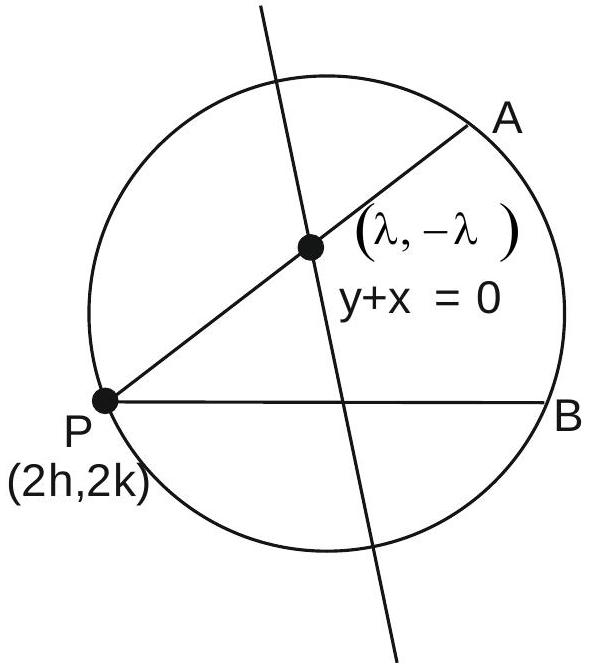
\includegraphics[max width=\textwidth, center]{2025_10_03_179189dc5202c17e9f52g-04}

Equation of chord \(\Rightarrow \mathrm{T}=\mathrm{S}_{1}\)\\
\(\Rightarrow(\mathrm{x}-\mathrm{y}) \lambda-\frac{2 \mathrm{~h}(\mathrm{x}+\lambda)}{2}-\frac{(2 \mathrm{k})(\mathrm{y}-\lambda)}{2}\)\\
\(=2 \lambda^{2}-2 \mathrm{~h}(\lambda)+2 \mathrm{k} \lambda\)\\
Now, \(\lambda(2 \mathrm{~h}, 2 \mathrm{k})\) satisfies the chord\\
\(\therefore(2 \mathrm{~h}-2 \mathrm{k}) \lambda-\mathrm{h}(\mathrm{x}+\lambda)-\mathrm{k}(\mathrm{y}-\lambda)\)\\
\(\Rightarrow 2 \lambda^{2}+4 \mathrm{k} \lambda-4 \mathrm{~h} \lambda+\mathrm{h} \lambda-\mathrm{k} \lambda+\mathrm{hx}+\mathrm{ky}=0\)\\
\(\Rightarrow 2 \lambda^{2}+\lambda(3 \mathrm{k}-3 \mathrm{~h})+\mathrm{ky}+\mathrm{hx}=0\)\\
\(\Rightarrow \mathrm{D}>0\)\\
\(\Rightarrow 9(\mathrm{k}-\mathrm{h})^{2}-8(\mathrm{ky}+\mathrm{hx})>0\)\\
\(\Rightarrow 9(\mathrm{k}-\mathrm{h})^{2}-8\left(2 \mathrm{k}^{2}+2 \mathrm{~h}^{2}\right)>0\)\\
\(\Rightarrow-7 \mathrm{k}^{2}-7 \mathrm{~h}^{2}-18 \mathrm{kh}>0\)\\
\(\Rightarrow 7 \mathrm{k}^{2}+7 \mathrm{~h}^{2}+18 \mathrm{kh}<0\)\\
\(\Rightarrow 7\left(\frac{1-\mathrm{a}}{4}\right)^{2}+7\left(\frac{1+\mathrm{a}}{4}\right)^{2}+18\left(\frac{1-\mathrm{a}^{2}}{16}\right)<0\)\\
\(\Rightarrow 7\left[\frac{2\left(1+\mathrm{a}^{2}\right)}{16}\right]+\frac{18\left(1-\mathrm{a}^{2}\right)}{16}<0, \quad \mathrm{a}^{2}=\mathrm{t}\)\\
\(\Rightarrow \frac{7}{8}(1+\mathrm{t})+\frac{18(1-\mathrm{t})}{16}<0\)\\
\(\Rightarrow \frac{14+14 \mathrm{t}+18-18 \mathrm{t}}{16}<0\)\\
\(\Rightarrow 4 \mathrm{t}>32\)\\
\(\mathrm{t}>8 \quad \mathrm{a}^{2}>8\)\\
67. Among the relations\\
\(S=\left\{(a, b): a, b \in \mathbb{R}-\{0\}, 2+\frac{a}{b}>0\right\}\)\\
And \(T=\left\{(a, b): a, b \in \mathbb{R}, a^{2}-b^{2} \in Z\right\}\),\\
(1) S is transitive but T is not\\
(2) T is symmetric but S is not\\
(3) Neither S nor T is transitive\\
(4) Both S and T are symmetric

Official Ans. by NTA (2)\\
Allen Ans. (2)\\
Sol. For relation \(\mathrm{T}=\mathrm{a}^{2}-\mathrm{b}^{2}=-\mathrm{I}\)\\
Then, \((\mathrm{b}, \mathrm{a})\) on relation R\\
\(\Rightarrow \mathrm{b}^{2}-\mathrm{a}^{2}=-\mathrm{I}\)\\
\(\therefore \mathrm{T}\) is symmetric\\
\(S=\left\{(a, b): a, b \in R-\{0\}, 2+\frac{a}{b}>0\right\}\)\\
\(2+\frac{\mathrm{a}}{\mathrm{b}}>0 \Rightarrow \frac{\mathrm{a}}{\mathrm{b}}>-2, \Rightarrow \frac{\mathrm{~b}}{\mathrm{a}}<\frac{-1}{2}\)\\
If \((b, a) \in S\) then\\
\(2+\frac{\mathrm{b}}{\mathrm{a}}\) not necessarily positive\\
\(\therefore \mathrm{S}\) is not symmetric\\
68. The equation\\
\(\mathrm{e}^{4 \mathrm{x}}+8 \mathrm{e}^{3 \mathrm{x}}+13 \mathrm{e}^{2 \mathrm{x}}-8 \mathrm{e}^{\mathrm{x}}+1=0, \mathrm{x} \in \mathrm{R}\) has:\\
(1) two solutions and both are negative\\
(2) no solution\\
(3) four solutions two of which are negative\\
(4) two solutions and only one of them is negative

Official Ans. by NTA (1)\\
Allen Ans. (1)

Sol. \(\mathrm{e}^{4 \mathrm{x}}+8 \mathrm{e}^{3 \mathrm{x}}+13 \mathrm{e}^{2 \mathrm{x}}-8 \mathrm{e}^{\mathrm{x}}+1=0\)\\
Let \(\mathrm{e}^{\mathrm{x}}=\mathrm{t}\)\\
Now, \(\mathrm{t}^{4}+8 \mathrm{t}^{3}+13 \mathrm{t}^{2}-8 \mathrm{t}+1=0\)\\
Dividing equation by \(t^{2}\),\\
\(\mathrm{t}^{2}+8 \mathrm{t}+13-\frac{8}{\mathrm{t}}+\frac{1}{\mathrm{t}^{2}}=0\)\\
\(\mathrm{t}^{2}+\frac{1}{\mathrm{t}^{2}}+8\left(\mathrm{t}-\frac{1}{\mathrm{t}}\right)+13=0\)\\
\(\left(\mathrm{t}-\frac{1}{\mathrm{t}}\right)^{2}+2+8\left(\mathrm{t}-\frac{1}{\mathrm{t}}\right)+13=0\)\\
Let \(\mathrm{t}-\frac{1}{\mathrm{t}}=\mathrm{z}\)\\
\(z^{2}+8 z+15=0\)\\
\((\mathrm{z}+3)(\mathrm{z}+5)=0\)\\
\(\mathrm{z}=-3\) or \(\mathrm{z}=-5\)\\
So, \(\mathrm{t}-\frac{1}{\mathrm{t}}=-3\) or \(\mathrm{t}-\frac{1}{\mathrm{t}}=-5\)\\
\(\mathrm{t}^{2}+3 \mathrm{t}-1=0\) or \(\mathrm{t}^{2}+5 \mathrm{t}-1=0\)\\
\(\mathrm{t}=\frac{-3 \pm \sqrt{13}}{2}\) or \(\mathrm{t}=\frac{-5 \pm \sqrt{29}}{2}\)\\
as \(\mathrm{t}=\mathrm{e}^{\mathrm{x}}\) so t must be positive,\\
\(\mathrm{t}=\frac{\sqrt{13}-3}{2}\) or \(\frac{\sqrt{29}-5}{2}\)\\
So, \(x=\ln \left(\frac{\sqrt{13}-3}{2}\right)\) or \(x=\ln \left(\frac{\sqrt{29}-5}{2}\right)\)\\
Hence two solution and both are negative.\\
69. The number of values of \(r \in\{p, q, \sim p, \sim q\}\) for which \(((\mathrm{p} \wedge \mathrm{q}) \Rightarrow(\mathrm{r} \vee \mathrm{q})) \wedge((\mathrm{p} \wedge \mathrm{r}) \Rightarrow \mathrm{q})\) is a tautology, is:\\
(1) 3\\
(2) 2\\
(3) 1\\
(4) 4

Official Ans. by NTA (2)\\
Allen Ans. (2)

Sol. \(\quad((\mathrm{p} \wedge \mathrm{q}) \Rightarrow(\mathrm{r} \vee \mathrm{q})) \wedge((\mathrm{p} \wedge \mathrm{r}) \Rightarrow \mathrm{q})\)\\
We know, \(p \Rightarrow q\) is equivalent to\\
\(\sim p \vee q\)\\
\((\sim(p \wedge q) v(r \vee q)) \wedge(\sim(p \wedge r)) \vee q))\)\\
\(\Rightarrow(\sim \mathrm{p} \vee \sim \mathrm{q} \vee \mathrm{r} \vee \mathrm{q}) \wedge(\sim \mathrm{p} \vee \sim \mathrm{r} \vee \mathrm{q})\)\\
\(\Rightarrow(\sim \mathrm{p} \vee \mathrm{r} \vee \mathrm{t}) \wedge(\sim \mathrm{p} \vee \sim \mathrm{r} \vee \mathrm{q})\)\\
\(\Rightarrow(\mathrm{t}) \wedge(\sim \mathrm{p} \vee \sim \mathrm{r} \vee \mathrm{q})\)\\
For this to be tautology, \((\sim p \vee \sim r \vee q)\) must be always true which follows for \(r=\sim p\) or \(r=q\).\\
70. Let \(\mathrm{f}: \mathbb{R}-\{2,6\} \rightarrow \mathbb{R}\) be real valued function defined as \(f(x)=\frac{x^{2}+2 x+1}{x^{2}-8 x+12}\). Then range of \(f\) is\\
(1) \(\left(-\infty,-\frac{21}{4}\right] \cup[0, \infty)\)\\
(2) \(\left(-\infty,-\frac{21}{4}\right) \cup(0, \infty)\)\\
(3) \(\left(-\infty,-\frac{21}{4}\right] \cup\left[\frac{21}{4}, \infty\right)\)\\
(4) \(\left(-\infty,-\frac{21}{4}\right] \cup[1, \infty)\)

Official Ans. by NTA (1)\\
Allen Ans. (1)\\
Sol. Let \(\mathrm{y}=\frac{\mathrm{x}^{2}+2 \mathrm{x}+1}{\mathrm{x}^{2}-8 \mathrm{x}+12}\)\\
By cross multiplying\\
\(\mathrm{yx}^{2}-8 \mathrm{xy}+12 \mathrm{y}-\mathrm{x}^{2}-2 \mathrm{x}-1=0\)\\
\(x^{2}(y-1)-x(8 y+2)+(12 y-1)=0\)\\
Case \(1, \mathrm{y} \neq 1\)\\
\(\mathrm{D} \geq 0\)\\
\(\Rightarrow(8 y+2)^{2}-4(y-1)(12 y-1) \geq 0\)\\
\(\Rightarrow \mathrm{y}(4 \mathrm{y}+21) \geq 0\)\\
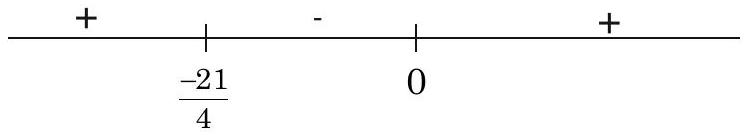
\includegraphics[max width=\textwidth, center]{2025_10_03_179189dc5202c17e9f52g-05}\\
\(\mathrm{y} \in\left(-\infty, \frac{-21}{4}\right] \cup[0, \infty)-\{1\}\)\\
Case 2, \(\mathrm{y}=1\)\\
\(\mathrm{x}^{2}+2 \mathrm{x}+1=\mathrm{x}^{2}-8 \mathrm{x}+12\)\\
\(10 \mathrm{x}=11\)\\
\(\mathrm{x}=\frac{11}{10} \quad\) So, y can be 1\\
Hence \(\mathrm{y} \in\left(-\infty, \frac{-21}{4}\right] \cup[0, \infty)\)\\
71. \(\lim _{\mathrm{x} \rightarrow \infty} \frac{(\sqrt{3 \mathrm{x}+1}+\sqrt{3 \mathrm{x}-1})^{6}+(\sqrt{3 \mathrm{x}+1}-\sqrt{3 \mathrm{x}-1})^{6}}{\left(\mathrm{x}+\sqrt{\mathrm{x}^{2}-1}\right)^{6}+\left(\mathrm{x}-\sqrt{\mathrm{x}^{2}-1}\right)^{6}} \mathrm{x}^{3}\)\\
(1) is equal to 9\\
(2) is equal to 27\\
(3) does not exist\\
(4) is equal to \(\frac{27}{2}\)

Official Ans. by NTA (2)\\
Allen Ans. (2)\\
Sol. \(\lim _{\mathrm{x} \rightarrow \infty} \frac{(\sqrt{3 \mathrm{x}+1}+\sqrt{3 \mathrm{x}-1})^{6}+(\sqrt{3 \mathrm{x}+1}-\sqrt{3 \mathrm{x}-1})^{6}}{\left(\mathrm{x}+\sqrt{\mathrm{x}^{2}-1}\right)^{6}+\left(\mathrm{x}-\sqrt{\mathrm{x}^{2}-1}\right)^{6}} \mathrm{x}^{3}\)\\
\(\lim _{x \rightarrow \infty} x^{3} \times\left\{\frac{x^{3}\left\{\left(\sqrt{3+\frac{1}{x}}+\sqrt{3-\frac{1}{x}}\right)^{6}+\left(\sqrt{3+\frac{1}{x}}-\sqrt{3-\frac{1}{x}}\right)^{6}\right\}}{x^{6}\left\{\left(1+\sqrt{1-\frac{1}{x^{2}}}\right)^{6}+\left(1-\sqrt{1-\frac{1}{x^{2}}}\right)^{6}\right\}}\right\}\)\\
\(=\frac{(2 \sqrt{3})^{6}+0}{2^{6}+0}=3^{3}=(27)\)\\
72. Let P be the plane, passing through the point \((1,-1,-5)\) and perpendicular to the line joining the points \((4,1,-3)\) and \((2,4,3)\). Then the distance of P from the point \((3,-2,2)\) is\\
(1) 6\\
(2) 4\\
(3) 5\\
(4) 7

Official Ans. by NTA (3)\\
Allen Ans. (3)

Sol. Equation of Plane :\\
\(2(x-1)-3(y+1)-6(z+5)=0\)\\
Or \(2 x-3 y-6 z=35\)\\
\(\Rightarrow\) Required distance \(=\)\\
\(\frac{|2(3)-3(-2)-6(2)-35|}{\sqrt{4+9+36}}\)\\
\(=5\)\\
73. The absolute minimum value, of the function \(\mathrm{f}(\mathrm{x})=\left|\mathrm{x}^{2}-\mathrm{x}+1\right|+\left[\mathrm{x}^{2}-\mathrm{x}+1\right], \quad\) where \(\quad[\mathrm{t}]\) denotes the greatest integer function, in the interval \([-1,2]\), is :\\
(1) \(\frac{3}{4}\)\\
(2) \(\frac{3}{2}\)\\
(3) \(\frac{1}{4}\)\\
(4) \(\frac{5}{4}\)

Official Ans. by NTA (1)\\
Allen Ans. (1)\\
Sol. \(\quad \mathrm{f}(\mathrm{x})=\left|\mathrm{x}^{2}-\mathrm{x}+1\right|+\left[\mathrm{x}^{2}-\mathrm{x}+1\right] ; \mathrm{x} \in[-1,2]\)

Let \(g(x)=x^{2}-x+1\)\\
\(=\left(x-\frac{1}{2}\right)^{2}+\frac{3}{4}\)\\
\(\because\left|\mathrm{x}^{2}-\mathrm{x}+1\right|\) and \(\left[\mathrm{x}^{2}-\mathrm{x}+2\right]\)

Both have minimum value at \(\mathrm{x}=1 / 2\)\\
\(\Rightarrow\) Minimum \(\mathrm{f}(\mathrm{x})=\frac{3}{4}+0\)\\
\(=\frac{3}{4}\)\\
74. Let the plane \(P: 8 \mathrm{x}+\alpha_{1} \mathrm{y}+\alpha_{2} \mathrm{z}+12=0\) be parallel to the line \(\mathrm{L}: \frac{\mathrm{x}+2}{2}=\frac{\mathrm{y}-3}{3}=\frac{\mathrm{z}+4}{5}\). If the intercept of P on the y -axis is 1 , then the distance between P and L is :\\
(1) \(\sqrt{14}\)\\
(2) \(\frac{6}{\sqrt{14}}\)\\
(3) \(\sqrt{\frac{2}{7}}\)\\
(4) \(\sqrt{\frac{7}{2}}\)

\section*{Official Ans. by NTA (1)}
Allen Ans. (1)\\
Sol. P: \(8 \mathrm{x}+\alpha_{1} \mathrm{y}+\alpha_{2} \mathrm{z}+12=0\)\\
\(\mathrm{L}: \frac{\mathrm{x}+2}{2}=\frac{\mathrm{y}-3}{3}=\frac{\mathrm{z}+4}{5}\)\\
\(\because \quad \mathrm{P}\) is parallel to L\\
\(\Rightarrow 8(2)+\alpha_{1}(3)+5\left(\alpha_{2}\right)=0\)\\
\(\Rightarrow 3 \alpha_{1}+5\left(\alpha_{2}\right)=-16\)\\
Also \(y\)-intercept of plane \(P\) is 1\\
\(\Rightarrow \alpha_{1}=-12\)\\
And \(\alpha_{2}=4\)\\
\(\Rightarrow\) Equation of plane P is \(2 \mathrm{x}-3 \mathrm{y}+\mathrm{z}+3=0\)\\
\(\Rightarrow\) Distance of line L from Plane P is\\
\(=\left|\frac{0-3(6)+1+3}{\sqrt{4+9+1}}\right|\)\\
\(=\sqrt{14}\)\\
75. The foot of perpendicular from the origin O to a plane P which meets the co-ordinate axes at the points \(\mathrm{A}, \mathrm{B}, \mathrm{C}\) is \((2, \mathrm{a}, 4), \mathrm{a} \in \mathrm{N}\). If the volume of the tetrahedron OABC is 144 unit \(^{3}\), then which of the following points is NOT on P?\\
(1) \((2,2,4)\)\\
(2) \((0,4,4)\)\\
(3) \((3,0,4)\)\\
(4) \((0,6,3)\)

\section*{Official Ans. by NTA (3)}
Allen Ans. (3)

Sol. Equation of Plane:

\[
\begin{aligned}
& (2 \hat{\mathrm{i}}+\mathrm{aj}+4 \hat{\mathrm{k}}) \cdot[(\mathrm{x}-2) \hat{\mathrm{i}}+(\mathrm{y}-\mathrm{a}) \hat{\mathrm{j}}+(\mathrm{z}-4) \hat{\mathrm{k}}]=0 \\
& \Rightarrow 2 \mathrm{x}+\mathrm{ay}+4 \mathrm{z}=20+\mathrm{a}^{2} \\
& \Rightarrow \mathrm{~A} \equiv\left(\frac{20+\mathrm{a}^{2}}{2}, 0,0\right) \\
& \mathrm{B} \equiv\left(0, \frac{20+\mathrm{a}^{2}}{\mathrm{a}}, 0\right) \\
& \mathrm{C} \equiv\left(0,0, \frac{20+\mathrm{a}^{2}}{4}\right) \\
& \Rightarrow \text { Volume of tetrahedron } \\
& =\frac{1}{6}[\overrightarrow{\mathrm{a}} \overrightarrow{\mathrm{~b}} \overrightarrow{\mathrm{c}}] \\
& =\frac{1}{6} \overrightarrow{\mathrm{a}} \cdot(\overrightarrow{\mathrm{~b}} \times \overrightarrow{\mathrm{c}}) \\
& \Rightarrow \frac{1}{6}\left(\frac{20+\mathrm{a}^{2}}{2}\right) \cdot\left(\frac{20+\mathrm{a}^{2}}{\mathrm{a}}\right) \cdot\left(\frac{20+\mathrm{a}^{2}}{4}\right)=144 \\
& \Rightarrow\left(20+\mathrm{a}^{2}\right)^{3}=144 \times 48 \times \mathrm{a} \\
& \Rightarrow \mathrm{a}=2
\end{aligned}
\]

\(\Rightarrow\) Equation of plane is \(2 x+2 y+4 z=24\)\\
Or \(\mathrm{x}+\mathrm{y}+2 \mathrm{z}=12\)\\
\(\Rightarrow(3,0,4) \quad\) Not lies on the Plane \(x+y+2 z=12\)\\
76. Let the mean and standard deviation of marks of class A of 100 students be respectively 40 and \(\alpha(>0)\), and the mean and standard deviation of marks of class \(B\) of \(n\) students be respectively 55 and \(30-\alpha\). If the mean and variance of the marks of the combined class of \(100+n\) students are respectively 50 and 350 , then the sum of variances of classes A and B is:\\
(1) 500\\
(2) 650\\
(3) 450\\
(4) 900

Official Ans. by NTA (1)\\
Allen Ans. (1)

Sol. D

A+B\\
\(\overline{\mathrm{x}}=50\)\\
\(\sigma^{2}=350\)\\
\(100+\mathrm{n}\)\\
\(\overline{\mathrm{x}}=\frac{100 \times 40+55 \mathrm{n}}{100+\mathrm{n}}\)\\
\(5000+50 n=4000+55 n\)\\
\(1000=5 \mathrm{n}\)\\
\(\mathrm{n}=200\)\\
\(\sigma_{1}{ }^{2}=\frac{\sum \mathrm{x}_{\mathrm{i}}{ }^{2}}{100}-40^{2}\)\\
\(\sigma_{2}{ }^{2}=\frac{\sum \mathrm{x}_{\mathrm{j}}{ }^{2}}{100}-55^{2}\)\\
\(350=\sigma^{2}=\frac{\sum \mathrm{x}_{\mathrm{i}}{ }^{2}+\sum \mathrm{x}_{\mathrm{j}}{ }^{2}}{300}-(\overline{\mathrm{x}})^{2}\)\\
\(350=\frac{\left(1600+\alpha^{2}\right) \times 100+\left[(30-\alpha)^{2}+3025\right] \times 200}{300}-(50)^{2}\)\\
\(2850 \times 3=\alpha^{2}+2(30-\alpha)^{2}+1600+6050\)\\
\(8550=\alpha^{2}+2(30-\alpha)^{2}+7650\)\\
\(\alpha^{2}+2(30-\alpha)^{2}=900\)\\
\(\alpha^{2}-40 \alpha+300=0\)\\
\(\alpha=10,30\)\\
\(\sigma_{1}{ }^{2}+\sigma_{2}{ }^{2}=10^{2}+20^{2}=500\)\\
77. Let : \(\vec{a}=\hat{i}+2 \hat{j}+3 \hat{k}, \vec{b}=\hat{i}-\hat{j}+2 \hat{k}\) and \(\vec{c}=5 \hat{i}-3 \hat{j}+3 \hat{k}\) be there vectors. If \(\vec{r}\) is a vector such that, \(\vec{r} \times \vec{b}=\vec{c} \times \vec{b}\) and \(\vec{r} \cdot \vec{a}=0\). Then \(25|\overrightarrow{\mathrm{r}}|^{2}\) is equal to\\
(1) 449\\
(2) 336\\
(3) 339\\
(4) 560

Official Ans. by NTA (3)

Allen Ans. (3)\\
Sol. \(\vec{a}=\hat{i}+2 \hat{j}+3 \hat{k}\)\\
\(\overrightarrow{\mathrm{b}}=\hat{\mathrm{i}}-\hat{\mathrm{j}}+2 \hat{\mathrm{k}}\)\\
\(\overrightarrow{\mathrm{c}}=\hat{5 \mathrm{i}}-3 \hat{\mathrm{j}}+3 \hat{\mathrm{k}}\)\\
\((\overrightarrow{\mathrm{r}}-\overrightarrow{\mathrm{c}}) \times \overrightarrow{\mathrm{b}}=0, \overrightarrow{\mathrm{r}} \cdot \overrightarrow{\mathrm{a}}=0\)\\
\(\Rightarrow \overrightarrow{\mathrm{r}}-\overrightarrow{\mathrm{c}}=\lambda \overrightarrow{\mathrm{b}}\)\\
Also, \((\overrightarrow{\mathrm{c}}+\lambda \overrightarrow{\mathrm{b}}) \cdot \overrightarrow{\mathrm{a}}=0\)\\
\(\Rightarrow \overrightarrow{\mathrm{a}} \cdot \overrightarrow{\mathrm{c}}+\lambda(\overrightarrow{\mathrm{a}} \cdot \overrightarrow{\mathrm{b}})=0\)\\
\(\therefore \lambda=\frac{\overrightarrow{\mathrm{a}} \cdot \overrightarrow{\mathrm{c}}}{\overrightarrow{\mathrm{a}} \cdot \overrightarrow{\mathrm{b}}}=\frac{-8}{5}\)\\
\(\vec{r}=\frac{5(5 \hat{i}-3 \hat{i}+3 \hat{k})-8(\hat{i}-\hat{j}+2 \hat{k})}{5}\)\\
\(\overrightarrow{\mathrm{r}}=\frac{17 \hat{\mathrm{i}}-7 \hat{\mathrm{j}}+\hat{\mathrm{k}}}{5}\)\\
\(|\overrightarrow{\mathrm{r}}|^{2}=\frac{1}{25}(289+50)\)\\
\(25|\vec{r}|^{2}=339\)\\
78. Let H be the hyperbola, whose foci are \((1 \pm \sqrt{2}, 0)\) and eccentricity is \(\sqrt{2}\). Then the length of its lat us rectum is \(\_\_\_\_\) .\\
(1) 2\\
(2) 3\\
(3) \(\frac{5}{2}\)\\
(4) \(\frac{3}{2}\)

Official Ans. by NTA (1)\\
Allen Ans. (1)\\
Sol. \(\quad 2 \mathrm{ae}=|(1+\sqrt{2})-(1+\sqrt{2})|=2 \sqrt{2}\)\\
\(\mathrm{ae}=\sqrt{2}\)\\
\(\mathrm{a}=1\)\\
\(\Rightarrow \mathrm{b}=1 \quad \because \mathrm{e}=\sqrt{2} \Rightarrow\) Hyperbola is rectangular\\
\(\Rightarrow\) L.R \(=\frac{2 \mathrm{~b}^{2}}{\mathrm{a}}=2\)\\
79. Let \(\alpha>0\). If \(\int_{0}^{\alpha} \frac{\mathrm{x}}{\sqrt{\mathrm{x}+\alpha}-\sqrt{\mathrm{x}}} \mathrm{dx}=\frac{16+20 \sqrt{2}}{15}\), then \(\alpha\) is equal to :\\
(1) 2\\
(2) 4\\
(3) \(\sqrt{2}\)\\
(4) \(2 \sqrt{2}\)

\section*{Official Ans. by NTA (1)}
Allen Ans. (1)\\
Sol. After rationalising

\[
\begin{aligned}
& \int_{0}^{\alpha} \frac{\mathrm{x}}{\alpha}(\sqrt{\mathrm{x}+\alpha}+\sqrt{\mathrm{x}}) \\
& \int_{0}^{\alpha} \frac{1}{\alpha}\left[(\mathrm{x}+\alpha)^{3 / 2}-\alpha(\mathrm{x}+\alpha)^{1 / 2}+\mathrm{x}^{3 / 2}\right] \\
&\left.\frac{1}{\alpha}\left[\frac{2}{5}(\mathrm{x}+\alpha)^{5 / 2}-\alpha \frac{2}{3}(\mathrm{x}+\alpha)^{3 / 2}+\frac{2}{5} \mathrm{x}^{5 / 2}\right]\right|_{0} ^{\alpha} \\
&= \frac{1}{\alpha}\left(\frac{5}{2}(2 \alpha)^{5 / 2}-\frac{2 \alpha}{3}(2 \alpha)^{3 / 2}+\frac{2}{5} \alpha^{5 / 2}-\frac{2}{5} \alpha^{5 / 2}+\frac{2}{3} \alpha^{5 / 2}\right) \\
&= \frac{1}{\alpha}\left(\frac{2^{7 / 2} \alpha^{5 / 2}}{5} \frac{2^{5 / 2} \alpha^{5 / 2}}{3}+\frac{2}{3} \alpha^{5 / 2}\right) \\
&= \alpha^{3 / 2}\left(\frac{2^{7 / 2}}{5}-\frac{2^{5 / 2}}{3}+\frac{2}{3}\right) \\
&= \frac{\alpha^{3 / 2}}{15}(24 \sqrt{2}-20 \sqrt{2}+10)=\frac{\alpha^{3 / 2}}{15}(4 \sqrt{2}+10)
\end{aligned}
\]

Now,\\
\(\frac{\alpha^{3 / 2}}{15}(4 \sqrt{2}+10)=\frac{16+20 \sqrt{2}}{15}\)\\
\(\Rightarrow \alpha=2\)\\
80. The complex number \(z=\frac{i-1}{\cos \frac{\pi}{3}+i \sin \frac{\pi}{3}}\) is equal to:\\
(1) \(\sqrt{2}\left(\cos \frac{5 \pi}{12}+\mathrm{i} \sin \frac{5 \pi}{12}\right)\)\\
(2) \(\cos \frac{\pi}{12}-i \sin \frac{\pi}{12}\)\\
(3) \(\sqrt{2}\left(\cos \frac{\pi}{12}+i \sin \frac{\pi}{12}\right)\)\\
(4) \(\sqrt{2} \mathrm{i}\left(\cos \frac{5 \pi}{12}-\mathrm{i} \sin \frac{5 \pi}{12}\right)\)

\section*{Official Ans. by NTA (1)}
Allen Ans. (1)\\
Sol. \(Z=\frac{i-1}{\cos \frac{\pi}{3}+i \sin \frac{\pi}{3}}=\frac{i-1}{\frac{1}{2}+\frac{\sqrt{3}}{2} i}\)\\
\(=\frac{\mathrm{i}-1}{\frac{1}{2}+\frac{\sqrt{3}}{2} \mathrm{i}} \times \frac{\frac{1}{2}-\sqrt{\frac{3}{2} \mathrm{i}}}{\frac{1}{2}-\sqrt{3 / 2} \mathrm{i}}=\frac{\sqrt{3}-1}{2}+\frac{\sqrt{3}+1}{2} \mathrm{i}\)\\
Apply polar form,\\
\(\mathrm{r} \cos \theta=\frac{\sqrt{3}-1}{2}\)\\
\(\mathrm{r} \sin \theta=\frac{\sqrt{3}+1}{2}\)\\
Now, \(\tan \theta=\frac{\sqrt{3}+1}{\sqrt{3}-1}\)\\
So, \(\quad \theta=\frac{5 \pi}{12}\)\\
81. The Coefficient of \(\mathrm{x}^{-6}\), in the expansion of \(\left(\frac{4 \mathrm{x}}{5}+\frac{5}{2 \mathrm{x}^{2}}\right)^{9}\), is \(\_\_\_\_\)\\
Official Ans. by NTA (5040)\\
Allen Ans. (5040)

Sol: \(\left(\frac{4 \mathrm{x}}{5}+\frac{5}{2 \mathrm{x}^{2}}\right)^{9}\),\\
Now, \(\mathrm{T}_{\mathrm{r}+1}={ }^{9} \mathrm{C}_{\mathrm{r}} \cdot\left(\frac{4 \mathrm{x}}{5}\right)^{9-\mathrm{r}}\left(\frac{5}{2 \mathrm{x}^{2}}\right)^{\mathrm{r}}\)\\
\(={ }^{9} \mathrm{C}_{\mathrm{r}} \cdot\left(\frac{4}{5}\right)^{9-\mathrm{r}}\left(\frac{5}{2}\right)^{\mathrm{r}} \cdot \mathrm{x}^{9-3 \mathrm{r}}\)\\
Coefficient of \(\mathrm{x}^{-6}\) i.e. \(9-3 \mathrm{r}=-6 \Rightarrow \mathrm{r}=5\)\\
So, Coefficient of \(\mathrm{x}^{-6}={ }^{9} \mathrm{C}_{5}\left(\frac{4}{5}\right)^{4} \cdot\left(\frac{5}{2}\right)^{5}=5040\)\\
82. Let the area of the region\\
\(\left\{(\mathrm{x}, \mathrm{y}):|2 \mathrm{x}-1| \leq \mathrm{y} \leq\left|\mathrm{x}^{2}-\mathrm{x}\right|, 0 \leq \mathrm{x} \leq 1\right\}\) be\\
A.

Then \((6 \mathrm{~A}+11)^{2}\) is equal to \(\_\_\_\_\) .

Official Ans. by NTA (125)\\
Allen Ans. (125)\\
Sol: \(\mathrm{y} \geq|2 \mathrm{x}-1|, \mathrm{y} \leq\left|\mathrm{x}^{2}-\mathrm{x}\right|\)\\
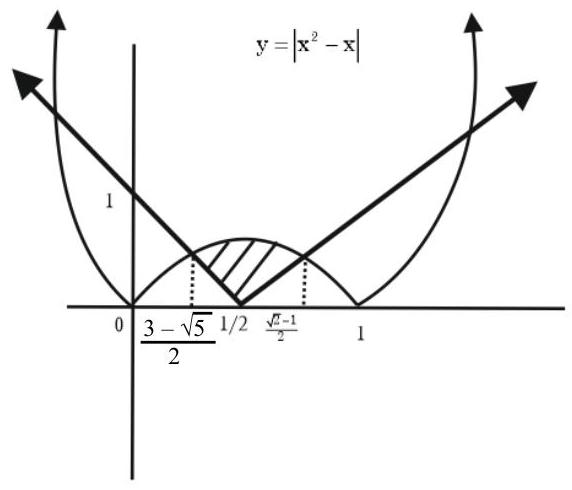
\includegraphics[max width=\textwidth, center]{2025_10_03_179189dc5202c17e9f52g-10}

Both curve are symmetric about \(\mathrm{x}=\frac{1}{2}\) Hence\\
\(A=2 \int_{\frac{3-\sqrt{5}}{2}}^{\frac{1}{2}}\left(\left(x-x^{2}\right)-(1-2 x)\right) d x\)\\
\(A=2 \int_{\frac{3-\sqrt{5}}{2}}^{\frac{1}{2}}\left(-x^{2}+3 x-1\right) d x=2\left(\frac{-x^{3}}{3}+\frac{3}{2} x^{2}-x\right)_{\frac{3-\sqrt{5}}{2}}^{\frac{1}{2}}\)\\
On solving \(6 \mathrm{~A}+11=5 \sqrt{5}\)\\
\((6 \mathrm{~A}+11)^{2}=125\)\\
83. If \({ }^{2 n+1} P_{n-1}:{ }^{2 n-1} P_{n}=11: 21\), then \(n^{2}+n+15\) is equal to:

Official Ans. by NTA (45)\\
Allen Ans. (45)\\
Sol: \(\frac{(2 n+1)!(n-1)!}{(n+2)!(2 n-1)!}=\frac{11}{21}\)\\
\(\Rightarrow \frac{(2 n+1)(2 n)}{(n+2)(n+1) n}=\frac{11}{21}\)\\
\(\Rightarrow \frac{2 \mathrm{n}+1}{(\mathrm{n}+1)(\mathrm{n}+2)}=\frac{11}{42}\)\\
\(\Rightarrow \mathrm{n}=5\)\\
\(\Rightarrow \mathrm{n}^{2}+\mathrm{n}+15=25+5+15=45\)\\
84. If the constant term in the binomial expansion of \(\left(\frac{x^{\frac{5}{2}}}{2}-\frac{4}{x^{\ell}}\right)^{9}\) is -84 and the Coefficient of \(x^{-3 \ell}\) is\\
\(2^{\alpha} \beta\), where \(\beta<0\) is an odd number, Then \(|\alpha \ell-\beta|\) is equal to \(\_\_\_\_\)\\
Official Ans. by NTA (98)\\
Allen Ans. (98)\\
Sol. In, \(\left(\frac{x^{\frac{5}{2}}}{2}-\frac{4}{x^{\ell}}\right)^{9}\)\\
\(\mathrm{T}_{\mathrm{r}+1}={ }^{9} \mathrm{C}_{\mathrm{r}} \frac{\left(\mathrm{x}^{5 / 2}\right)^{9-\mathrm{r}}}{2^{9-\mathrm{r}}}\left(\frac{-4}{\mathrm{x}^{\ell}}\right)^{\mathrm{r}}\)\\
\(=(-1)^{\mathrm{r}} \frac{{ }^{9} \mathrm{C}_{\mathrm{r}}}{2^{9-\mathrm{r}}} 4^{\mathrm{r}} \mathrm{X}^{\frac{45}{2}-\frac{5 \mathrm{r}}{2}-\mathrm{lr}}\)\\
\(=45-5 r-21 r=0\)\\
\(r=\frac{45}{5+21}\)

Now, according to the question, \((-1)^{\mathrm{r}} \frac{{ }^{9} \mathrm{C}_{\mathrm{r}}}{2^{9-\mathrm{r}}} 4^{\mathrm{r}}=-84\)\\
\(=(-1)^{\mathrm{r}}{ }^{9} \mathrm{C}_{\mathrm{r}} 2^{3 \mathrm{r}-9}=21 \times 4\)\\
Only natural value of \(r\) possible if \(3 r-9=0\)\\
\(\mathrm{r}=3\) and \({ }^{9} \mathrm{C}_{3}=84\)\\
\(\therefore 1=5\) from equation (1)\\
Now, coefficient of \(\mathrm{x}^{-31}=\mathrm{x}^{\frac{45}{2}-\frac{5 \mathrm{r}}{2}-\mathrm{lr}}\) at \(1=5\), gives \(\mathrm{r}=5\)\\
\(\therefore{ }^{9} \mathrm{c}_{5}(-1) \frac{4^{5}}{2^{4}}=2^{\alpha} \times \beta\)\\
\(=-63 \times 2^{7}\)\\
\(\Rightarrow \alpha=7, \beta=-63\)\\
\(\therefore\) value of \(|\alpha \ell-\beta|=98\)\\
85. Let \(\vec{a}, \vec{b}, \vec{c}\) be three vectors such that \(|\vec{a}|=\sqrt{31}, 4|\vec{b}|=|\vec{c}|=2\) and \(2(\vec{a} \times \vec{b})=3(\vec{c} \times \vec{a})\). If the angle between \(\vec{b}\) and \(\vec{c}\) is \(\frac{2 \pi}{3}\), then \(\left(\frac{\overrightarrow{\mathrm{a}} \times \overrightarrow{\mathrm{c}}}{\overrightarrow{\mathrm{a}} \cdot \overrightarrow{\mathrm{b}}}\right)^{2}\) is equal to \(\_\_\_\_\) .

Official Ans. by NTA (3)\\
Allen Ans. (3)\\
Sol. \(2(\vec{a} \times \vec{b})=3(\vec{c} \times \vec{a})\)\\
\(\overrightarrow{\mathrm{a}} \times(2 \overrightarrow{\mathrm{~b}}+3 \overrightarrow{\mathrm{c}})=0\)\\
\(\overrightarrow{\mathrm{a}}=\lambda(2 \overrightarrow{\mathrm{~b}}+3 \overrightarrow{\mathrm{c}})\)\\
\(|\overrightarrow{\mathrm{a}}|^{2}=\lambda^{2}|2 \overrightarrow{\mathrm{~b}}+3 \overrightarrow{\mathrm{c}}|^{2}\)\\
\(|\overrightarrow{\mathrm{a}}|^{2}=\lambda^{2}\left(4|\overrightarrow{\mathrm{~b}}|^{2}+9|\overrightarrow{\mathrm{c}}|^{2}+12 \overrightarrow{\mathrm{~b}} \cdot \overrightarrow{\mathrm{c}}\right)\)\\
\(31=31 \lambda^{2} \Rightarrow \lambda= \pm 1\)\\
\(\overrightarrow{\mathrm{a}}= \pm(2 \overrightarrow{\mathrm{~b}}+3 \overrightarrow{\mathrm{c}})\)\\
\(\frac{|\overrightarrow{\mathrm{a}} \times \overrightarrow{\mathrm{c}}|}{|\overrightarrow{\mathrm{a}} \cdot \overrightarrow{\mathrm{b}}|}=\frac{2|\overrightarrow{\mathrm{~b}} \times \overrightarrow{\mathrm{c}}|}{2 \overrightarrow{\mathrm{~b}} \cdot \overrightarrow{\mathrm{~b}}+3 \overrightarrow{\mathrm{c}} \cdot \overrightarrow{\mathrm{b}}}\)\\
\(|\overrightarrow{\mathrm{b}} \times \overrightarrow{\mathrm{c}}|^{2}=|\overrightarrow{\mathrm{b}}|^{2}|\overrightarrow{\mathrm{c}}|^{2}-(\overrightarrow{\mathrm{b}} . \overrightarrow{\mathrm{c}})^{2}=\frac{3}{4}\)\\
\(\frac{|\overrightarrow{\mathrm{a}} \times \overrightarrow{\mathrm{c}}|}{|\overrightarrow{\mathrm{a}} \cdot \overrightarrow{\mathrm{b}}|}=\frac{2 \times \frac{\sqrt{3}}{2}}{2 \cdot \frac{1}{4}-\frac{3}{2}}=-\sqrt{3}\)\\
\(\left(\frac{\overrightarrow{\mathrm{a}} \times \overrightarrow{\mathrm{c}}}{\overrightarrow{\mathrm{a}} \cdot \overrightarrow{\mathrm{b}}}\right)^{2}=3\)\\
86. Let S be the set of all \(\mathrm{a} \in \mathrm{N}\) such that the area of the triangle formed by the tangent at the point \(\mathrm{P}(\mathrm{b}, \mathrm{c}), \mathrm{b}, \mathrm{c} \in \mathrm{N}\), on the parabola \(\mathrm{y}^{2}=2 \mathrm{ax}\) and the lines \(\mathrm{x}=\mathrm{b}, \mathrm{y}=0\) is 16 unit \(^{2}\), then \(\sum_{\mathrm{a} \in \mathrm{S}} \mathrm{a}\) is equal to \(\_\_\_\_\) .\\
Official Ans. by NTA (146)\\
Allen Ans. (146)\\
Sol.\\
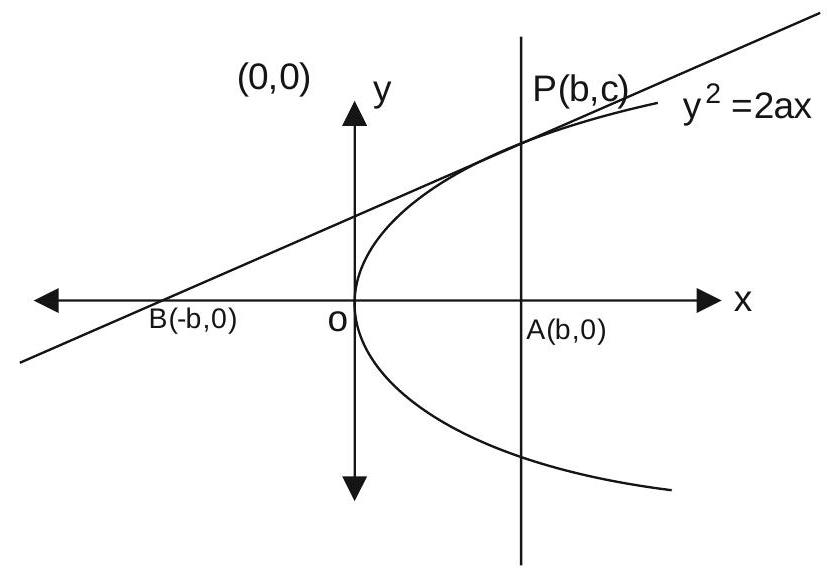
\includegraphics[max width=\textwidth, center]{2025_10_03_179189dc5202c17e9f52g-11}

As \(\mathrm{P}(\mathrm{b}, \mathrm{c})\) lies on parabola so \(\mathrm{c}^{2}=2 \mathrm{ab}\)

Now equation of tangent to parabola \(y^{2}=2 a x\) in point\\
form is \(\mathrm{yy}_{1}=2 \mathrm{a} \frac{\left(\mathrm{x}+\mathrm{x}_{1}\right)}{2},\left(\mathrm{x}_{1}, \mathrm{y}_{1}\right)=(\mathrm{b}, \mathrm{c})\)\\
\(\Rightarrow \mathrm{yc}=\mathrm{a}(\mathrm{x}+\mathrm{b})\)\\
For point B , put \(\mathrm{y}=0\), now \(\mathrm{x}=-\mathrm{b}\)\\
So, area of \(\triangle \mathrm{PBA}, \frac{1}{2} \times \mathrm{AB} \times \mathrm{AP}=16\)\\
\(\Rightarrow \frac{1}{2} \times 2 \mathrm{~b} \times \mathrm{c}=16\)\\
\(\Rightarrow \mathrm{bc}=16\)\\
As \(b\) and \(c\) are natural number so possible values of \((\mathrm{b}, \mathrm{c})\) are \((1,16),(2,8),(4,4),(8,2)\) and \((16,1)\)\\
Now from equation (1) \(a=\frac{c^{2}}{2 b}\) and \(a \in N\), so values of (b,c) are (1,16), (2,8) and (4,4) now values of are 128, 16 and 2.\\
Hence sum of values of a is 146 .\\
87. The sum\\
\(1^{2}-2.3^{2}+3.5^{2}-4.7^{2}+5.9^{2}-\ldots \ldots . .+15.29^{2}\) is \(\_\_\_\_\) .\\
Official Ans. by NTA (6952 )\\
Allen Ans. (6952)\\
Separating odd placed and even placed terms we get\\
\(\mathrm{S}=\left(1.1^{2}+3.5^{2}+\ldots .15 .(29)^{2}\right)-\left(2.3^{2}+4.7^{2}\right.\)\\
\(+\ldots .+14 .(27)^{2}\)\\
\(S=\sum_{n=1}^{8}(2 n-1)(4 n-3)^{2}-\sum_{n=1}^{7}(2 n)(4 n-1)^{2}\)\\
Applying summation formula we get\\
\(=29856-22904=6952\)\\
88. Let A be the event that the absolute difference between two randomly choosen real numbers in the sample space \([0,60]\) is less than or equal to a . If \(\mathrm{P}(\mathrm{A})=\frac{11}{36}\), then a is equal to \(\_\_\_\_\) .\\
Official Ans. by NTA (10)\\
Allen Ans. (10)\\
Sol: \(|\mathrm{x}-\mathrm{y}|<\mathrm{a} \Rightarrow-\mathrm{a}<\mathrm{x}-\mathrm{y}<\mathrm{a}\)\\
\(\Rightarrow \mathrm{x}-\mathrm{y}<\mathrm{a}\) and \(\mathrm{x}-\mathrm{y}>-\mathrm{a}\)\\
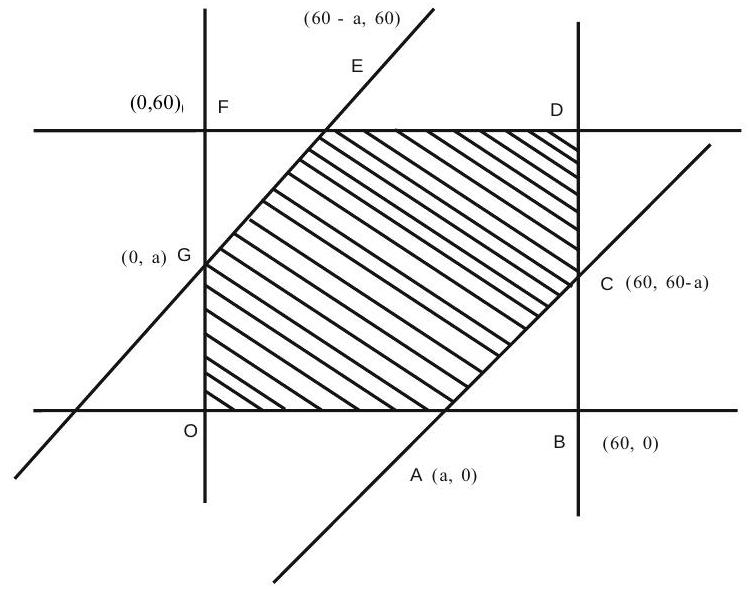
\includegraphics[max width=\textwidth, center]{2025_10_03_179189dc5202c17e9f52g-12}\\
\(\mathrm{P}(\mathrm{A})=\frac{\operatorname{ar}(\mathrm{OACDEG})}{(\mathrm{OBDF})}\)\\
\(=\frac{\operatorname{ar}(\mathrm{OBDF})-\operatorname{ar}(\mathrm{ABC})-\operatorname{ar}(\mathrm{EFG})}{\operatorname{ar}(\mathrm{OBDF})}\)\\
\(\Rightarrow \frac{11}{36}=\frac{(60)^{2}-\frac{1}{2}(60-\mathrm{a})^{2}-\frac{1}{2}(60-\mathrm{a})^{2}}{3600}\)\\
\(\Rightarrow 1100=3600-(60-\mathrm{a})^{2}\)\\
\(\Rightarrow \quad(60-\mathrm{a})^{2}=2500 \Rightarrow 60-\mathrm{a}=50\)\\
\(\Rightarrow \mathrm{a}=10\)\\
89. Let \(\mathrm{A}=\left[\mathrm{a}_{\mathrm{ij}}\right], \mathrm{a}_{\mathrm{ij}} \in \mathrm{Z} \cap[0,4], 1 \leq \mathrm{i}, \mathrm{j} \leq 2\). The number of matrices A such that the sum of all entries is a prime number \(\mathrm{p} \in(2,13)\) is\\
\(\_\_\_\_\) .\\
Official Ans. by NTA ( 196)\\
Allen Ans. (204 )\\
As given \(\mathrm{a}+\mathrm{b}+\mathrm{c}+\mathrm{d}=3\) or 5 or 7 or 11\\
if sum \(=3\)\\
\(\left(1+\mathrm{x}+\mathrm{x}^{2}+\ldots . .+\mathrm{x}^{4}\right)^{4} \rightarrow \mathrm{x}^{3}\)\\
\(\left(1-x^{5}\right)^{4}(1-x)^{-4} \rightarrow x^{3}\)\\
\(\therefore{ }^{4+3-1} \mathrm{C}_{3}={ }^{6} \mathrm{C}_{3}=20\)\\
If sum \(=5\)\\
\(\left(1-4 x^{5}\right)(1-x)^{-4} \rightarrow x^{5}\)\\
\(\Rightarrow{ }^{4+5-1} \mathrm{C}_{5}-4 \mathrm{x}^{4.4+0-1} \mathrm{C}_{0}={ }^{8} \mathrm{C}_{5}-4=52\)\\
If sum \(=7\)\\
\(\left(1-4 x^{5}\right)(1-x)^{-4} \rightarrow x^{7}\)\\
\(\Rightarrow{ }^{4+5-1} \mathrm{C}_{4}-{ }^{4.4+0-1} \mathrm{C}_{0}={ }^{8} \mathrm{C}_{5}-4=52\)\\
If sum \(=11\)

\[
\begin{aligned}
& \left(1-4 \mathrm{x}^{5}+6 \mathrm{x}^{10}\right)(1-\mathrm{x})^{-4} \rightarrow \mathrm{x}^{11} \\
\Rightarrow & { }^{4+11-1} \mathrm{C}_{11}-4 .{ }^{4+6-4} \mathrm{C}_{6}+6 .{ }^{4+1-1} \mathrm{C}_{1} \\
= & { }^{14} \mathrm{C}_{11}-4 .{ }^{9} \mathrm{C}_{6}+6.4=364-336+24=52 \\
\therefore & \text { Total matrices }=20+52+80+52=204
\end{aligned}
\]

\begin{enumerate}
  \setcounter{enumi}{89}
  \item Let A be a \(\mathrm{n} \times \mathrm{n}\) matrix such that \(|\mathrm{A}|=2\). If the determinant of the matrix \(\operatorname{Adj}\left(2 . \operatorname{Adj}\left(2 \mathrm{~A}^{-1}\right)\right)\). is \(2^{84}\), then n is equal to \(\_\_\_\_\) .\\
Official Ans. by NTA (5)\\
Allen Ans. (5)\\
Sol. \(\left|\operatorname{Adj}\left(2 \operatorname{Adj}\left(2 \mathrm{~A}^{-1}\right)\right)\right|\)\\
\(=\left|2 \operatorname{Adj}\left(\operatorname{Adj}\left(2 \mathrm{~A}^{-1}\right)\right)\right|^{n-1}\)\\
\(=2^{\mathrm{n}(\mathrm{n}-1)}\left|\operatorname{Adj}\left(2 \mathrm{~A}^{-1}\right)\right|^{\mathrm{n}-1}\)\\
\(=2^{\mathrm{n}(\mathrm{n}-1)}\left|\left(2 \mathrm{~A}^{-1}\right)\right|^{(\mathrm{n}-1)(\mathrm{n}-1)}\)\\
\(=2^{\mathrm{n}(\mathrm{n}-1)} 2^{\mathrm{n}(\mathrm{n}-1)(\mathrm{n}-1)}\left|\mathrm{A}^{-1}\right|^{(\mathrm{n}-1)(\mathrm{n}-1)}\)\\
\(=2^{\mathrm{n}(\mathrm{n}-1)+\mathrm{n}(\mathrm{n}-1)(\mathrm{n}-1)} \frac{1}{|\mathrm{~A}|^{(\mathrm{n}-1)^{2}}}\)\\
\(=\frac{2^{\mathrm{n}(\mathrm{n}-1)+\mathrm{n}(\mathrm{n}-1)(\mathrm{n}-1)}}{2^{(\mathrm{n}-1)^{2}}}\)\\
\(=2^{\mathrm{n}(\mathrm{n}-1)+\mathrm{n}(\mathrm{n}+1)^{2}-(\mathrm{n}-1)^{2}}\)\\
\(=2^{(\mathrm{n}-1)\left(\mathrm{n}^{2}-\mathrm{n}+1\right)}\)\\
Now, \(2^{(\mathrm{n}-1)\left(\mathrm{n}^{2}-\mathrm{n}+1\right)}\)\\
\(2^{(\mathrm{n}-1)\left(\mathrm{n}^{2}-\mathrm{n}+1\right)}=2^{84}\)\\
So, \(\mathrm{n}=5\)
\end{enumerate}

\end{document}